\documentclass[final]{beamer}

\usepackage[orientation=portrait, size=a0, scale=1.5, debug]{beamerposter}
\usepackage{booktabs}
\usepackage{dcolumn}
\usepackage{colortbl}
\usepackage{xcolor}
\usepackage{hyperref}
\usepackage{amsmath}
% \usepackage[absolute, showboxes, overlay]{textpos}
\usepackage[absolute, overlay]{textpos}
\usepackage{calc}
% \usepackage[colorgrid,texcoord]{eso-pic}
\usepackage[bibstyle=numeric,maxcitenames=6]{biblatex}

% \defaultfontfeatures{Mapping=tex-text}
\usepackage{pifont}
\usepackage{multicol}
\usepackage{algorithm}
\usepackage[noend]{algpseudocode} 
\usepackage{mathtools}
\usepackage{array}
\usepackage{color}
\usepackage[export]{adjustbox}
\usepackage{multirow}
\usepackage{dsfont}
\usepackage{bm}
\usepackage{xcolor}
\usepackage{marvosym,latexsym}
\usepackage{amssymb}
\usepackage{anyfontsize}
\usepackage{caption,subcaption}

\newcommand{\X}{\ensuremath{\mathbf{X}}}
\newcommand{\Y}{\ensuremath{\mathbf{Y}}}
%\newcommand{\x}{\ensuremath{\mathbf{x}}}
\newcommand{\y}{\ensuremath{\mathbf{y}}}

\newcommand{\SPN}{\mathcal{S}}
\newcommand{\Node}{\mathsf{N}}
\newcommand{\Leaf}{\mathsf{L}}
%\newcommand{\Node}{\mathcal{N}}
\newcommand{\SumNode}{\mathsf{S}}
\newcommand{\ProdNode}{\mathsf{P}}
\newcommand{\DistNode}{\mathsf{D}}
\newcommand{\Nodes}{\bm{\mathsf{N}}}
\newcommand{\DistNodes}{\bm{\mathsf{D}}}
\newcommand{\SumNodes}{\bm{\mathsf{S}}}
\newcommand{\ProdNodes}{\bm{\mathsf{P}}}

\newcommand{\ch}{\mathsf{ch}}
\newcommand{\scope}{\mathsf{sc}}

\newcommand{\w}{w}
\usepackage{wasysym}

% \newcolumntype{L}[1]{>{\raggedright\let\newline\\\arraybackslash\hspace{0pt}}m{#1}}
% \newcolumntype{C}[1]{>{\centering\let\newline\\\arraybackslash\hspace{0pt}}m{#1}}
% \newcolumntype{R}[1]{>{\raggedleft\let\newline\\\arraybackslash\hspace{0pt}}m{#1}}

\usetheme{spinaceto}

\addbibresource{referomnia.bib}

\usepackage{blindtext}

% \newcommand*\mccol[2]{\multicolumn{#1}{c}{#2}}
% \newcommand*\tmccol[2]{\mccol{#1}{\tiny\textsf{#2}}}
% \newcommand*\bmccol[2]{\mccol{#1}{\textbf{#2}}}
\newcommand{\argmax}{\operatornamewithlimits{argmax}}
\newcommand{\argmin}{\operatornamewithlimits{argmin}}
\newcommand{\nodeset}[1]{\bm{\mathsf{#1}}}
\newcommand{\cndbar}{\,|\,}
\newcommand{\x}{\mathbf{x}}

\newcommand{\comment}[3][\normalsize]{\begin{minipage}{1\linewidth}
          \raggedleft
          {
            $\color{violet}\boldsymbol\Rightarrow$
            #1
            {\emph{#2}}
          }
      \end{minipage}#3\\
}

\newcommand{\commenta}[3][\normalsize]{\hspace{50pt}\begin{minipage}{.9\linewidth}
          \raggedleft
          {
            % $\color{violet}\boldsymbol\Rightarrow$
            #1
            {\emph{#2}}
          }
      \end{minipage}#3\\
}

\newcommand{\commenti}[3][\normalsize]{\hspace{50pt}\begin{minipage}{.9\linewidth}
          \raggedleft
          {
            $\color{violet}\boldsymbol\Rightarrow$
            #1
            {\emph{#2}}
          }
      \end{minipage}#3\\
}

\newcommand{\commentia}[3][\normalsize]{\hspace{50pt}\begin{minipage}{.9\linewidth}
    \vspace{-20pt}
          \raggedleft
          {
            $\color{violet}\boldsymbol\Rightarrow$
            #1
            {\emph{#2}}
          }
      \end{minipage}#3\\
}


\definecolor{mpigreen-off} {RGB} {17, 102, 86}
\definecolor{mpigreen} {RGB} {0, 129, 122}

\DeclareMathOperator*{\EX}{\mathbb{E}}

\newcommand{\KL}{\ensuremath{\mathbb{K}\mathbb{L}}}
\newcommand{\VAR}{\ensuremath{\mathbb{VAR}}}
\newcommand{\HE}{\ensuremath{\mathbb{H}}}
\newcommand{\Li}{\ensuremath{\mathsf{L}}}
\newcommand{\R}{\ensuremath{\mathsf{R}}}
\newcommand{\xl}{\ensuremath{\x^{\Li}}}
\newcommand{\xr}{\ensuremath{\x^{\R}}}
\newcommand{\LR}{\ensuremath{\mathsf{LR}}}
\newcommand{\LC}{\ensuremath{\mathsf{LC}}}

\newcommand{\ouralgoname}{\ensuremath{\textsc{EC$_2$}}}
\newcommand{\ouralgomoment}{\ensuremath{\textsc{MC$_2$}}}


\newcommand{\Gen}{\ensuremath{p_{\theta}}}
\newcommand{\Disc}{\ensuremath{f_{\phi}}}


\newcommand{\EXPK}[1]{\ensuremath{\EX_{#1}(\Gen, \Disc)}}

\newcommand{\EXPGK}[3]{\ensuremath{\EX_{#1}(p_{#2}, g_{#3})}}

\newcommand{\flow}[2]{\ensuremath{\mathds{1}_{#1}(#2)}}

\newcommand{\pr}{\ensuremath{p_{\R}}}
\newcommand{\pl}{\ensuremath{p_{\Li}}}
\newcommand{\gr}{\ensuremath{g_{\R}}}
\newcommand{\gl}{\ensuremath{g_{\Li}}}

\DeclareMathOperator{\Var}{Var}

\definecolor{lacamlilac} {RGB} {107,93,153}
\definecolor{lacamlilac2} {RGB} {93, 109, 152}
\definecolor{lacamlightlilac} {RGB} {174, 166, 201}
\definecolor{lacamdarklilac} {RGB} {51, 10, 102}
\definecolor{lacamdarklilac5} {RGB} {51, 10, 102}
\colorlet{lacamdarklilac4} {lacamdarklilac5!80!}
\colorlet{lacamdarklilac3} {lacamdarklilac5!60!}
\colorlet{lacamdarklilac2} {lacamdarklilac5!40!}
\colorlet{lacamdarklilac1} {lacamdarklilac5!20!}
\definecolor{pink3} {HTML} {F06292}
\definecolor{lacamgold5} {RGB} {255, 87, 0}
\colorlet{lacamgold4} {lacamgold5!80!}
\colorlet{lacamgold3} {lacamgold5!60!}
\colorlet{lacamgold2} {lacamgold5!40!}
\colorlet{lacamgold1} {lacamgold5!20!}
\definecolor{violet} {RGB} {119, 111, 178}
\definecolor{petroil2} {RGB} {36, 165, 175}
\definecolor{petroil4} {RGB} {30, 132, 149}
\definecolor{petroil6} {RGB} {23, 101, 115}
\definecolor{gold1} {RGB} {254, 176, 52}
\definecolor{gold2} {RGB} {255, 130, 0}
\definecolor{gold4} {RGB} {250, 100, 0}
\definecolor{gold6} {RGB} {245, 90, 0}
\definecolor{gold8} {RGB} {212, 62, 0}
\definecolor{gold10} {RGB} {180, 29, 0}
\definecolor{greentue} {RGB} {50, 152, 101}

\definecolor{lacamoil5}{rgb}{0.13, 0.67, 0.8}
\colorlet{lacamoil4} {lacamoil5!80!}
\colorlet{lacamoil3} {lacamoil5!60!}
\colorlet{lacamoil2} {lacamoil5!40!}

\definecolor{tomato0} {HTML} {EF9A9A}
\definecolor{tomato1} {HTML} {F44336}
\definecolor{tomato2} {HTML} {E53935}
\definecolor{tomato3} {HTML} {D32F2F}
\definecolor{tomato4} {HTML} {C62828}
\definecolor{tomato5} {HTML} {B71C1C}

\definecolor{peas1} {HTML} {009688}
\definecolor{peas2} {HTML} {00897B}
\definecolor{peas3} {HTML} {00796B}
\definecolor{peas4} {HTML} {00695C}
\definecolor{peas5} {HTML} {004D40}

\definecolor{bgrey0} {HTML} {78909C}
\definecolor{bgrey1} {HTML} {607D8B}
\definecolor{bgrey2} {HTML} {546E7A}
\definecolor{bgrey3} {HTML} {455A64}
\definecolor{bgrey4} {HTML} {37474F}
\definecolor{bgrey5} {HTML} {263238}

\definecolor{olive0} {HTML} {C5E1A5}
\definecolor{olive1} {HTML} {AED581}
\definecolor{olive2} {HTML} {9CCC65}
\definecolor{olive3} {HTML} {8BC34A}
\definecolor{olive4} {HTML} {7CB342}
\definecolor{olive5} {HTML} {689F38}

\definecolor{pink0} {HTML} {FCE4EC}
\definecolor{pink1} {HTML} {F8BBD0}
\definecolor{pink2} {HTML} {F48FB1}
\definecolor{pink3} {HTML} {F06292}
\definecolor{pink4} {HTML} {EC407A}
\definecolor{pink5} {HTML} {FF80AB}

\definecolor{brown0} {HTML} {D7CCC8}
\definecolor{brown1} {HTML} {BCAAA4}
\definecolor{brown2} {HTML} {A1887F}
\definecolor{brown3} {HTML} {8D6E63}
\definecolor{brown4} {HTML} {795548}
\definecolor{brown5} {HTML} {6D4C41}
\definecolor{brown6} {HTML} {5D4037}

\definecolor{yellow0} {HTML} {CDDC39}
\definecolor{yellow1} {HTML} {9E9D24}
\definecolor{yellow2} {HTML} {74741b}
\definecolor{yellow3} {HTML} {FFBD2A}
\definecolor{yellow4} {HTML} {FFB000}
\definecolor{yellow5} {HTML} {FFD600}
\definecolor{yellow6} {HTML} {D6C67B}

\definecolor{wwine} {HTML} {cccaa9}
\definecolor{rwine} {HTML} {770a2d}
\definecolor{abagreen} {HTML} {2ca02c}
\definecolor{abapink} {HTML} {e377c2}
\definecolor{abagray} {HTML} {7f7f7f}
\definecolor{abayellow} {HTML} {bcbd22}
\definecolor{ababrown} {HTML} {8c564b}

\newcommand{\headercol}{bgrey2}
\newcommand{\expcol}{gold8}
\newcommand{\expcols}{gold8}

\usepackage{tikz}
\usetikzlibrary{circuits.logic.US}
\usetikzlibrary{shapes.misc}
\usetikzlibrary{shapes.arrows}
\usetikzlibrary{arrows,shapes.geometric}
\usetikzlibrary{patterns,calc,backgrounds}
\usetikzlibrary{trees}

\tikzstyle{nnf}=[
>=latex, thick, >=stealth,
% font=\small,
auto,scale=0.9,every node/.style={scale=0.9}
]
\tikzstyle{nnfnode}=[
  line width=.01\textwidth,%1.0pt,
draw
]
\tikzstyle{nnfand}=[
  nnfnode, and gate, rotate=90
]
\tikzstyle{nnfor}=[
  nnfnode, or gate, rotate=90
]
\tikzstyle{nnf2or}=[
  nnfor, inputs=nn
]
\tikzstyle{nnf2and}=[
  nnfand, inputs=nn
]
\tikzstyle{nnf3or}=[
  nnfor, inputs=nnn, scale=0.75
]
\tikzstyle{nnf4and}=[
  nnfand, inputs=nnnn, scale=0.65
]
\tikzstyle{nnfedge}=[
    line width=.009\textwidth%0.9
]
\tikzstyle{nnfterm}=[
  draw,fill=gray!10,inner sep=.05\textwidth, %font=\small
]
\definecolor{hotcolor}{rgb}{0.85,0.0,0.0}
\tikzstyle{hot}=[
  draw=hotcolor, line width=.01\textwidth%1.1pt
]
\tikzstyle{hotparam}=[
  text=hotcolor
]


% \newcommand{\htt}[2][yellow]{\mathchoice%
%   {\colorbox{#1}{\textcolor{white}{$\displaystyle{#2}$}}}%
%   {\colorbox{#1}{\textcolor{white}{$\textstyle{#2}$}}}%
%   {\colorbox{#1}{\textcolor{white}{$\scriptstyle{#2}$}}}%
%   {\colorbox{#1}{\textcolor{white}{$\scriptscriptstyle{#2}$}}}}%

% \newcommand{\htttext}[2][yellow]{{\colorbox{#1}{\textcolor{white}{#2\vphantom{\"Ag}}}}}

% \newcommand{\hbs}[1]{\hspace*{#1\baselineskip}}

% \newcommand{\httm}[3][.2]{\ifmmode\mathchoice%
%   {\colorbox{#2}{\hbs{#1}\textcolor{white}{$\displaystyle{#3}$}\hbs{#1}}}%
%   {\colorbox{#2}{\hbs{#1}\textcolor{white}{$\textstyle{#3}$}\hbs{#1}}}%
%   {\colorbox{#2}{\hbs{#1}\textcolor{white}{$\scriptstyle{#3}$}\hbs{#1}}}%
%   {\colorbox{#2}{\hbs{#1}\textcolor{white}{$\scriptscriptstyle{#3}$}\hbs{#1}}}
%   \else{\colorbox{#2}{\hbs{#1}\textcolor{white}{#3\vphantom{\"Aq}$\mathop{\vphantom{\int}}$}\hbs{#1}}}\fi} 

% \newcommand{\htt}[2][yellow]{\httm[.1]{#1}{#2}}

% \newcommand{\httb}[2][yellow]{\htt[#1]{\ifmmode\mathbf{#2}\else\textbf{#2}\fi}}

% \newcommand{\authorbox}[4][140pt]{\begin{minipage}{#1}{\fontsize{40}{30}\selectfont\raggedright\textbf{{
%           #2}}\\[-20pt]
%     \hspace{10pt}\scriptsize{\emph{#3}}}\end{minipage}}

% \newcommand{\affiliationbox}[5][160pt]{\parbox[t]{200pt}{\begin{minipage}[t]{#1}\vspace{0pt}
%     \raggedright\includegraphics[width=0.98\linewidth]{#2}\end{minipage}\begin{minipage}[t]{10pt}\vspace{5pt}\footnotesize[#5]\end{minipage}\\[10pt]
%   % {\footnotesize[#4]}
%   \parbox[t]{170pt}{\linespread{.7}
%     \raggedright
%     \footnotesize{#3}
%     \\[2pt]
%     \scriptsize{\emph{#4}}
%     % \fontsize{20}{2}
%     % {#3}
    
%   }}
%   }

\def\restrict#1{\mkern 1mu \vrule height 1.3ex\mkern2mu #1}

\makeatletter
\def\maketag@@@#1{\hbox{\m@th\normalfont\small#1}\hspace{30pt}}
\makeatother


\newcolumntype{R}[2]{
  >{\adjustbox{angle=#1,lap=\width-(#2)}\bgroup}
  l
  <{\egroup}
}

\newcommand*\rot{\multicolumn{1}{R{45}{1em}}}
% \newcommand*\rot{\rotatebox{60}}

% 
% custom colors
\definecolor{untractable_red}{RGB}{209, 25, 25}
\definecolor{tractable_green}{RGB}{0, 153, 51}

% \newcommand{\cmark}{\ding{51}}%
% \newcommand{\xmark}{\ding{55}}

% \newcommand{\summark}{\tiny\textcolor{lacamlilac}{$\boldsymbol{\oplus}$}}
% \newcommand{\prodmark}{\tiny\textcolor{lacamlilac}{$\boldsymbol{\otimes}$}}

\newcommand{\sqbull}{\fcolorbox{\expcols}{\expcols}{\rule{0pt}{10pt}\rule{10pt}{0pt}}}

% \setbeamertemplate{itemize item}{\raisebox{.21ex}{\hbox{\summark}\hspace{0pt}}}
% \setbeamertemplate{itemize subitem}{\raise .2ex\hbox{\prodmark}\hspace{0pt}}
% \setbeamertemplate{itemize
%   subsubitem}{\textcolor{lacamlilac}{$\oplus$}}

\setbeamertemplate{itemize item}{\raisebox{.21ex}{\hbox{\sqbull}\hspace{0pt}}}
\setbeamertemplate{itemize subitem}{\raise .2ex\hbox{\sqbull}\hspace{0pt}}
\setbeamertemplate{itemize
  subsubitem}{\textcolor{lacamlilac}{$\sqbull$}}
% \setbeamersize{text margin left = 10em}

% \setbeamertemplate{bibliography item}{\hspace{10pt}\raise
%   .2ex\hbox{\tiny\textcolor{lacamlilac}{$\boldsymbol{\oplus}$}}\insertbiblabel}
\setbeamertemplate{bibliography item}{\insertbiblabel}


\setbeamertemplate{headline}{}

% \addbibresource{../referomnia/referomnia.bib}



\begin{document}

% \institute{Università degli Studi di Bari}
% \department{Dipartimento di Informatica}
% \laboratory{LACAM}
% \group{Machine Learning}

% \institutelogo{\includegraphics[width=25pt]{figures/unibaba}}
% \lablogo{\includegraphics[width=35pt]{figures/lacam}}


% {
%   \setbeamertemplate{headline}{}
%   \setbeamertemplate{footline}{}
%   \begin{textblock}
%     \titlepage
%   \end{textblock}
% }

\newcommand{\hmargin}{22.5mm}
\newcommand{\vmargin}{22.5mm}
\textblockorigin{\hmargin}{\vmargin}

\setlength{\TPHorizModule}{1cm}
\setlength{\TPVertModule}{1cm}

\setlength\fboxsep{5pt}

%
% TODO: generalize this
\newlength{\posterwidth}
\newlength{\posterheight}
\setlength{\posterwidth}{1189mm}
\setlength{\posterheight}{841mm - 2\hmargin}

\newcommand{\ncols}{3}
\newcommand{\scalefactor}{1.4}
\newlength{\colwidth}
\setlength{\colwidth}{\posterwidth/\ncols}

\newlength{\colhpoint}
\setlength{\leftmargini}{35pt}


\begin{frame}{}
  %
  % title
  % \textblockcolour{header}
  \begin{textblock}{78}(0, 0)
    \usebeamerfont{section name}
    \Huge
    \fontsize{115}{105}\selectfont
    \httm[.3]{\expcol}{{On Tractable Computation}}\\[-5pt]
    \httm[.3]{\expcol}{{of Expected Predictions}}
  \end{textblock}
  %
  % authors
  \begin{textblock}{300}(0, 13)
    \authorbox[280pt]{\emph{Pasha Khosravi}}{}{}
    \authorbox[260pt]{{YooJung Choi}}{}{}
    \authorbox[220pt]{{Yitao Liang}}{}{}
    \authorbox[300pt]{{Antonio Vergari}}{}{}
    \authorbox[360pt]{{Guy Van den Broeck}}{}{}\\[-15pt]
    \emph{\{pashak,\ yjchoi,\ yliang,\ aver,\ guyvdb\}@cs.ucla.edu}
  \end{textblock}
    
  %
  % affiliations
  \begin{textblock}{10}(66, 0)
    \begin{minipage}[t]{400pt}\vspace{0pt}
      \raggedleft
\includegraphics[width=0.8\linewidth]{figures/ucla-logo}\end{minipage}\\[25pt]
    \hfill\begin{minipage}[t]{400pt}\vspace{0pt}
      \hfill\raggedleft
\includegraphics[width=0.6\linewidth]{figures/starai}\end{minipage}
  \end{textblock}

  
  
\begin{textblock}{17}(0, 18)
    \usebeamerfont{section name}
    \htt[\expcols]{{Motivation}}
\end{textblock}
  
\begin{textblock}{38}(0, 22)
  \large
  In presence of uncertainty, one needs to
  probabilistically reason about the \emph{\textbf{expected predictions}} of
  regressors and classifiers.

 \vspace{25pt}
 Expected Prediction appears in many interesting applications such as  \emph{handling missing values, fairness, and data analysis}. 

 \vspace{25pt}
 More generally, we want to \emph{\textbf{compute {the $k$-th moment}}} of a predictive model $f$ w.r.t.\ the feature distribution $p$:
 \begin{equation*}
        M_k(f,p) \triangleq \EX\nolimits_{\x \sim p(\x)} \left[ (f(\x))^k
        \right]
        \label{eq:mom}
  \end{equation*} 

\end{textblock}

\begin{textblock}{17}(0, 39.5)
    \usebeamerfont{section name}
    \htt[\expcols]{{Complexity results}}
\end{textblock}

\begin{textblock}{39}(0, 43.5)
  \large
  In general, this computation is not tractable. It is hard even for simple pairs of models naive Bayes and logistic regression~\cite{Khosravi2019}.

  \vspace{20pt}

  We consider \emph{\textbf{expressive models}} represented as \emph{\textbf{probabilistic circuits}}~\cite{Darwiche2003}:\\[10pt]
  \vspace{20pt}
  \hfill\begin{minipage}{0.95\linewidth}
  \begin{itemize}
    \setlength{\itemsep}{10pt}
  % \item arbitrary $f$ and $p$ \\[-10pt]
  %   \commenti{\#P-Hard}{}
  % \item $f$ is a {\emph{logistic regressor}} and $p$
  %   \emph{{Naive Bayes}}\\[-50pt] %$\color{violet}\boldsymbol\Rightarrow$
  %   \commenti{{\textbf{NP-Hard}}~\cite{Khosravi2019}}{}    
    % \\[-10pt]
    % \commenti{NP-Hard}{}
%$\color{violet}\boldsymbol\Rightarrow$ \emph{\color{tractable_green} \textbf{polytime algorithm}}!
  \item $f$ is a \emph{{regression circuit}} and $p$ is a \emph{{generative
        circuit}}\par with {\emph{different vtree}}\\[-60pt]
    \commenti{{\color{untractable_red}\textbf{proved \#P-Hard! {\large\frownie{}}}}}{}
%$\color{violet}\boldsymbol\Rightarrow$ 
  \item $f$ is a \emph{{classification circuit}} and $p$ is a \emph{{generative
        circuit}}\par {\emph{even with same vtree}}\\[-50pt]
    \commenti{{\color{untractable_red}\textbf{proved NP-Hard! {\large\frownie{}}}}  {}}{}
    %$\color{violet}\boldsymbol\Rightarrow$
    %\emph{\color{untractable_red}\textbf{proved NP-Hard}}!
  \item  $f$ is a \emph{{regression circuit}} and $p$ is a \emph{{generative
        circuit}}\par with the {\emph{same vtree}}\\[-60pt]
    \commenti{ {\color{tractable_green} \textbf{polytime algorithm! {\large\smiley{}}}}}{}
  \end{itemize}  
  \end{minipage}

\end{textblock}


%\begin{textblock}{17}(0, 65)
\begin{textblock}{17}(0, 67.5)
    \usebeamerfont{section name}
    \htt[\expcols]{{Generative and discriminative circuits}}\\[-5pt]
    %\htt[\expcols]{{circuits}}
\end{textblock}


\begin{textblock}{38}(0, 71.5)
  \large
  For $p$ we consider a generative
circuit like a \emph{\textbf{probabilistic sentential decision diagram}} (\textbf{PSDD})~\cite{Kisa2014}
\begin{equation*}
p_n(\x) =
 \begin{cases}
    \mathds{1}_{n}(\x)  &\text{if $n$ is a leaf,}\\
    \pl(\xl) \cdot \pr(\xr)&\text{if $n$ is an AND gate,}\\
    \sum_{i \in\ch(n)} \theta_i p_i(\x) &\text{if $n$ is an OR gate.}
\end{cases}   
\label{eq:prob-circuit-semantics}
\end{equation*}
\comment{structured decomposable, smooth}{}\vspace{30pt}

For regression, we employ a \emph{\textbf{regression circuit}} (\textbf{RC}), defining: 
\begin{equation*}
g_{m}(\x) =
 \begin{cases}
    0 &\text{if $m$ is a leaf,}\\
    \gl(\xl) + \gr(\xr) &\text{if $m$ is an AND gate,}\\
    \sum\nolimits_{j\in \mathsf{ch}(m)} \mathds{1}_{j}(\x)(\phi_{j} + g_{j}(\x)) &\text{if $m$ is an OR gate.}
\end{cases} 
\label{eq:glc-semantics}
\end{equation*}

\vspace{40pt}
For classification, we use a \emph{\textbf{logistic circuit}}
(\textbf{LC})~\cite{LiangAAAI19}, modeling $f(\x) = \gamma\circ g_r(\x) = 1 / (1+e^{-g_r(\x)})$.\par

\comment{structured decomposable, smooth, deterministic}{}\vspace{30pt}

\end{textblock}

\begin{textblock}{38}(42, 14)
  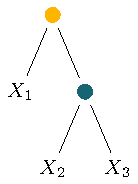
\includegraphics[width=.15\columnwidth]{figures/vtree}\hspace{80pt}
  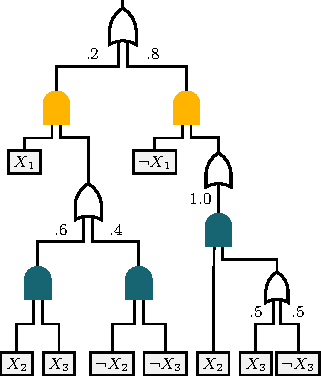
\includegraphics[width=.3\columnwidth]{figures/psdd}\hspace{80pt}
  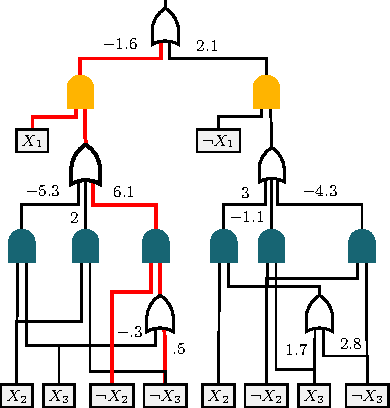
\includegraphics[width=.35\columnwidth]{figures/lgc}\\[30pt]
  \commenta{A vtree (left), and a generative (center) and
    discriminative circuit (right) conforming to it.
    % Corresponding AND  gates match by color,
    Determinism is shown by a red ``hot'' wire.}{}
\end{textblock}



\begin{textblock}{17}(42, 33)
    \usebeamerfont{section name}
    %\normalsize
    \htt[\expcols]{{Recursive moment decomposition}}
\end{textblock}
\begin{textblock}{38}(42, 37)
  \large
  Recursively "pushes down" the computation to their children.
  
 \begin{center}
      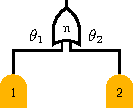
\includegraphics[width=.20\columnwidth]{figures/recursive_example_p.pdf}\hspace{80pt}
      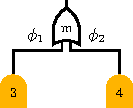
\includegraphics[width=.20\columnwidth]{figures/recursive_example_f.pdf}\hspace{80pt}
 \end{center}
 \commenta{For example, for the pair of OR nodes $(n,m)$ the computation involves solving subproblems $(1,3), (1,4), (2, 3), (3,4)$.}

\vspace{40pt}
The $k^{\text{th}}$ moments are computed \textbf{\emph{exactly}} in $O(k^2\cdot  |p_n|\cdot |g_m|)$.
\end{textblock}

\begin{textblock}{17}(42, 53)
    \usebeamerfont{section name}
    \htt[\expcols]{{Reasoning with missing values}}
\end{textblock}
\begin{textblock}{38}(42, 57)
  \large
  Given partial evidence $\x^{o}$ we want to compute
  \begin{align*}
    \EX\nolimits_{\x^{m}\sim p(\x^{m}|\x^{o})}\left[f(\x^m \x^o)\right] = 
    \frac{1}{p(\x^{o})}\EX\nolimits_{\x^{m}\sim p(\x^{m}, \x^{o})}\left[f(\x^m \x^o)\right]
    \label{eq:exp-miss-ii}
  \end{align*}

    \vspace{30pt}
    \textbf{Regression:} Expected prediction outperforms many imputation strategies such as mean, median, MPE, and MICE.
    
    \begin{center}
        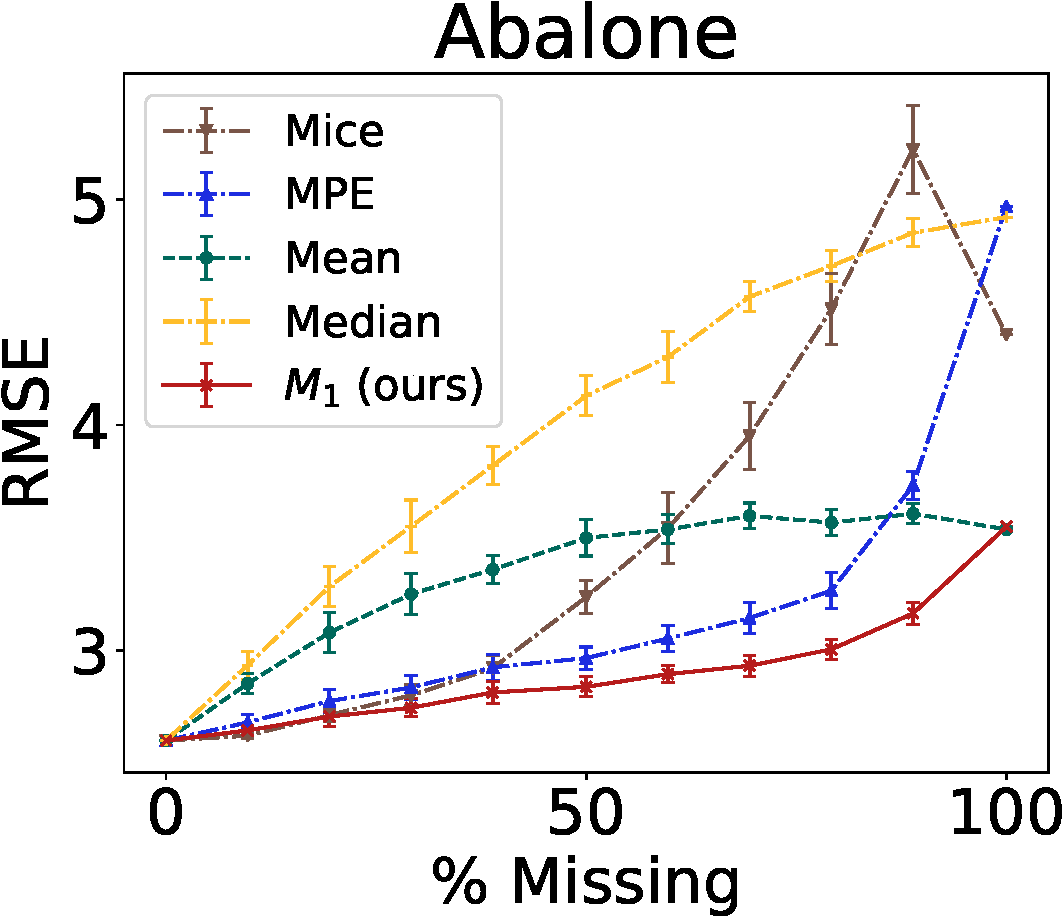
\includegraphics[width=.25\columnwidth]{figures/abalone_try-I_sqrtmse_plot_merged-crop.pdf}\hspace{20pt}
        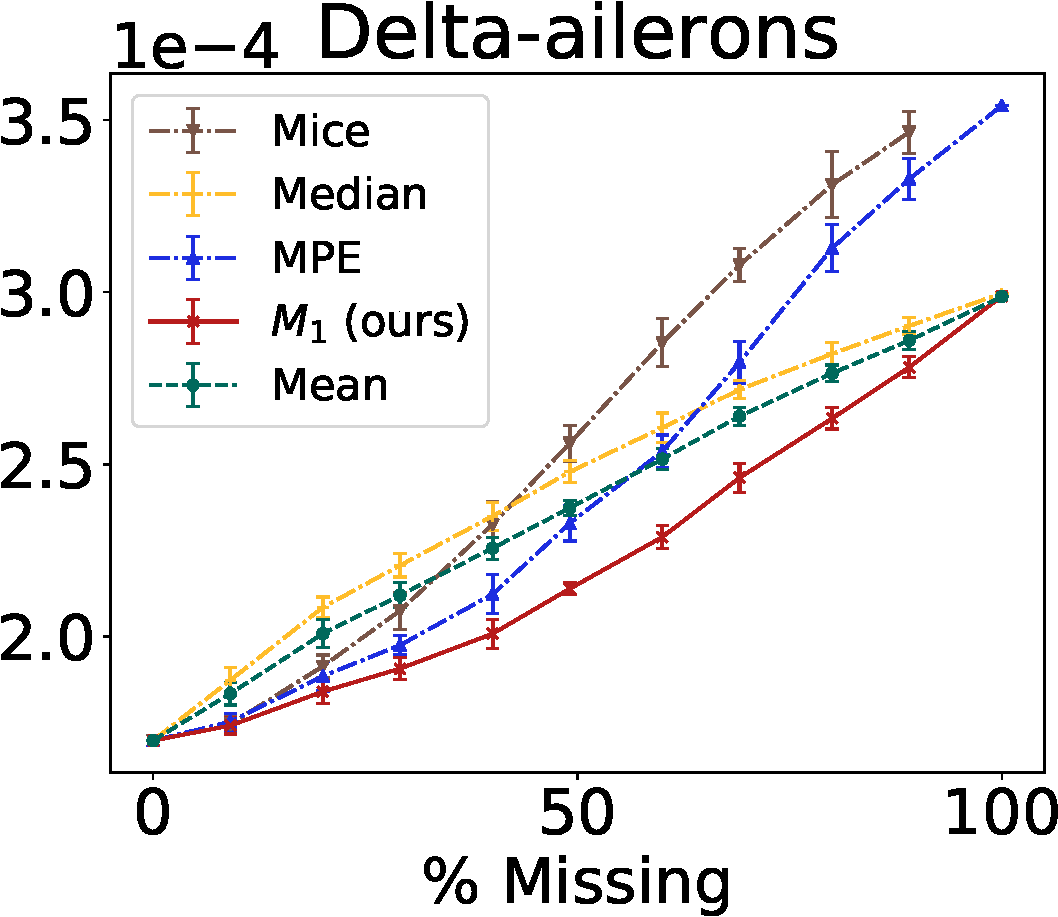
\includegraphics[width=.25\columnwidth]{figures/delta-ailerons_try-I_sqrtmse_plot_merged-crop.pdf}\hspace{20pt}
        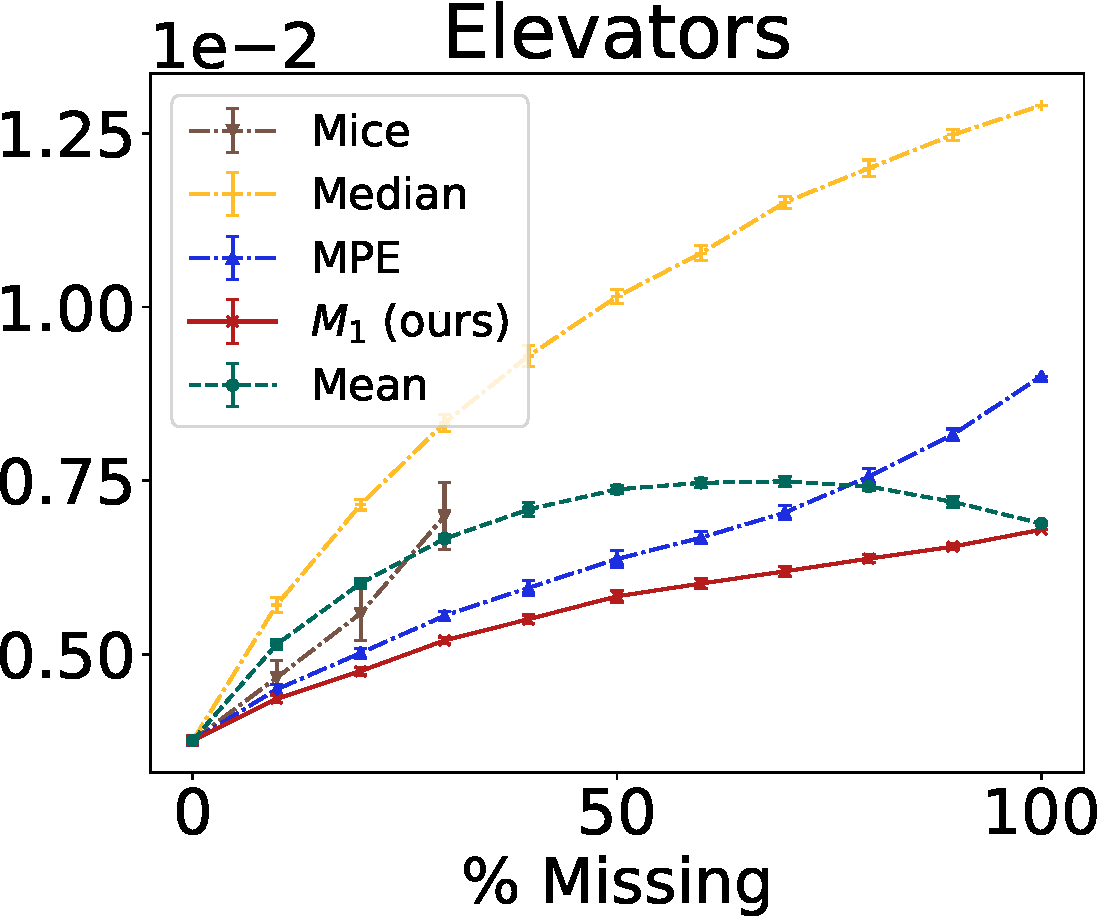
\includegraphics[width=.25\columnwidth]{figures/elevators_try-I_sqrtmse_plot_merged-crop.pdf}\\[5pt]
    \end{center}

    \vspace{20pt}
    \textbf{Classification:} We provide an approximation involving Taylor series and moments of $g$, which also outperforms several baselines (see paper). 

\end{textblock}
  
\begin{textblock}{17}(42, 84)
    \usebeamerfont{section name}
    %\normalsize
    \htt[\expcols]{{Analyze behaviour of predictive models}}
\end{textblock}

\begin{textblock}{38}(42, 88)
    \large
    \textbf{Insurance dataset}: yearly health insurance costs of people living in the USA.
    
    \textbf{Q1:} “Difference of insurance costs between smokers and non smokers?”
    \begin{equation*}
        M_1(f,\ p(.\ \vert\ \textit{Smoker})) - M_1(f,\ p(.\ \vert\ \textit{Non Smoker})) = 22,614
    \end{equation*}
    
    \vspace{20pt}
    
    \textbf{Q2:} "Is the predictive model    biased by gender?"
    \begin{equation*}
        M_1(f,\ p(.\ \vert\ \textit{Female})) - M_1(f,\ p(.\ \vert\ \textit{Male})) = 974
    \end{equation*}

    \vspace{20pt}
    
    \textbf{Q3:} "Expected cost of a female ($\mathsf{F}$) smokers ($\mathsf{S}$) with one child ($\mathsf{C}$)" living in southeast ($\mathsf{SE}$)? How about Std of the cost?"   
    \begin{align*}
       \mu &= M_1(f,p(.\ \vert\  \mathsf{F,S,C,SE})) &= 30,974 \\
        \sigma &= \sqrt{M_2(.) - (M_1(.))^2} &= 11,229
    \end{align*}
    
\end{textblock}

\begin{textblock}{17}(0, 104)
    \usebeamerfont{section name}
    %\normalsize
    \htt[\expcols]{\emph{References}}
\end{textblock}


  \begin{textblock}{38}(0, 107.8)
    \small
    \begin{multicols}{2}
    \setlength\bibitemsep{8pt}
    \printbibliography[heading=none]
    \end{multicols}
  \end{textblock}

  % 
  % footer
  \begin{textblock}{66}(0, 114.)
    \usebeamerfont{subtitle}
    \small
    \textbf{NeurIPS 2019}  -   Dec 2019, Vancouver, Canada\hfill
    % \textbf{Paper} - 
    % {\url{arxiv.org/abs/1807.09306}}\ \ $\cdotp$ \ \
    %     \textbf{Code} - 
    % {\url{github.com/probabilistic-learning/abda}}
  \end{textblock}
  
\end{frame}


\end{document}

%%% Local Variables:
%%% mode: latex
%%% TeX-engine: xetex
%%% TeX-master: t
%%% End:
